\section{Inference}
\label{inference}
%Given the motivation for this paper we suggest that inference should be incremental.  An incremental technique known as particle filtering has been explored in several non-parameteric Bayesian settings \cite{Fearnhead2004, Wood2007}.  

Proposing a generative model is only the first step in modeling discrete sequence data.  The process which generates real sequence data is normally unobserved and the form of the generative mechanism must be inferred.  The task of inference is to estimate the generative mechanism given data.

The sequential nature of the generative process suggests using a sequential Monte Carlo method (SMC) \cite{Doucet2001}.  In Algorithm~\ref{alg1} we show a SMC procedure for estimating a variant of the model introduced in Section~\ref{sec:sm} in which distributions are assumed to vary in the way developed in Section~\ref{sec:dhpyp}.  In this algorithm each particle consists of a set of occupied restaurants and a weight.  Each particle is updated incrementally for each observation in a streaming sequence.

The operation NextObservation() returns the next symbol in the sequence.  The variable $\bf(u)$ is the context in which the symbol $x$ was observed.  The ProposeRestaurantToDelete() method returns a restaurant sampled from a proposal distribution.  The FindRestaurant($\bf{u}$) returns a path from the restaurant $\G_{[]}$ to the restaurant $\G_{\bf{u}}$.  Finding the path requires descending the tree from the root and instantiating all necessary restaurants.  The set of instantiated restaurants in the particle is updated to reflect restaurants instantiated during the FindRestaurant($\bf{u}$) call.  The Seat($x,\bf{P}^k$) method returns the a priori probability of observing $x$ in the context $\bf{u}$ and a customer associated with the observation according the the posterior distribution over tables given the state of the particle and the observation $x$.  If the Seat() method sits the customer associated with $x$ at a new table it will also need to seat a customer in the parent restaurant.  This seating process may extend all the say up to the restaurant $\G_{[]}$.

%we propose makes inference using a particle filter approach straightforward. 

%A particle filter works by using a swarm of particles to approximate the posterior distribution over the model space conditional on observed data.  The approximation is represented as a weighted sample, each particle embodying a possible state of the model.  In view of a new data point the weight of each particle is adjusted to reflect the new information.  In the non-parameteric Bayesian setting, since the parameter space is growing as a function of the length of the data, values for new parameters must be incorporated into each particle.  New parameter values are produced through a proposal distribution which is taken into account when the weight of each particle is updated.  To make the inference more efficient proposal distributions are usually chosen to approximate the posterior distribution of the new parameter given the current set of observed data.

%We propose here an inferential procedure for the dependent memory-constrained hierarchical Pitman-Yor process model performed in the modified dependent Chinese restaurant franchise representation.  Using this representation, each observation corresponds to a customer seated in the appropriate restaurant.  The latent parameters in the model are the table at which each customer is seated and the restaurants which are deleted at each deletion step.  For the table assignments, a particle filter in this representation will, for each particle, seat the customer corresponding to the most recently observed data in the appropriate restaurant at a table produced from a proposal distribution.  Since seating a customer may indicate the presence of an additional customer in the parent restaurant, a table for a new customer may need to be proposed in the parent restaurant as well.  It is possible that customers will need to be seated all the way up the path until the restaurant corresponding to the distribution over symbols conditional on an empty context.  The proposal distribution we suggest for choosing a table for each customer is the posterior distribution conditional on the new observation and the current state of the particle.  Details of this inference scheme applied to the SM can be found in \cite{Gasthaus2010}.

\newcommand{\Restaurant}{R^{k}}
\newcommand{\Weight}{w^{k}}
\newcommand{\Context}{\mathbf{u}}
\newcommand{\Path}{\mathbf{P}^{k}}
\newcommand{\D}{\mathbf{d}}
\newcommand{\LongPath}{\{ \Restaurant_\Context, \Restaurant_{\pi(\Context)}, \dots, \Restaurant_{[]} \}}
\begin{algorithm}
\caption{Particle Filter}
\begin{algorithmic}[1]
\STATE Initialize $K$ particles $\{\{\Restaurant = \emptyset, \Weight = \frac{1}{K}\}\}_{k=1}^{K}$
\STATE Initialize $\Context = []$
\WHILE{true}
	\STATE $x \gets $ NextObservation()
	\STATE $\Context \gets \Context x$
	\FORALL {$k = 1,\dots,K$}
		\IF {$|\Restaurant| > $ maxRestaurants $ -\, 2 $}
			\STATE $\Restaurant_\D \gets $ ProposeRestaurantToDelete()
			\STATE $\Restaurant \gets \Restaurant \setminus \Restaurant_\D$
		\ENDIF
		\STATE $\LongPath \gets $ FindRestaurant($\Context$)
		\STATE $\Path \gets \LongPath$
		\STATE $\Restaurant \gets \Restaurant \cup \Path$
		\STATE $v^{k} \gets $ Seat($x, \Path$)
		\STATE $\Weight \gets v^{k}\Weight$
	\ENDFOR
	\STATE \# resample particles 
	\STATE \# predict
\ENDWHILE
\end{algorithmic}
\label{alg1}
\end{algorithm}


\begin{figure*}[t] 
	\begin{center}
		\scalebox{.4}{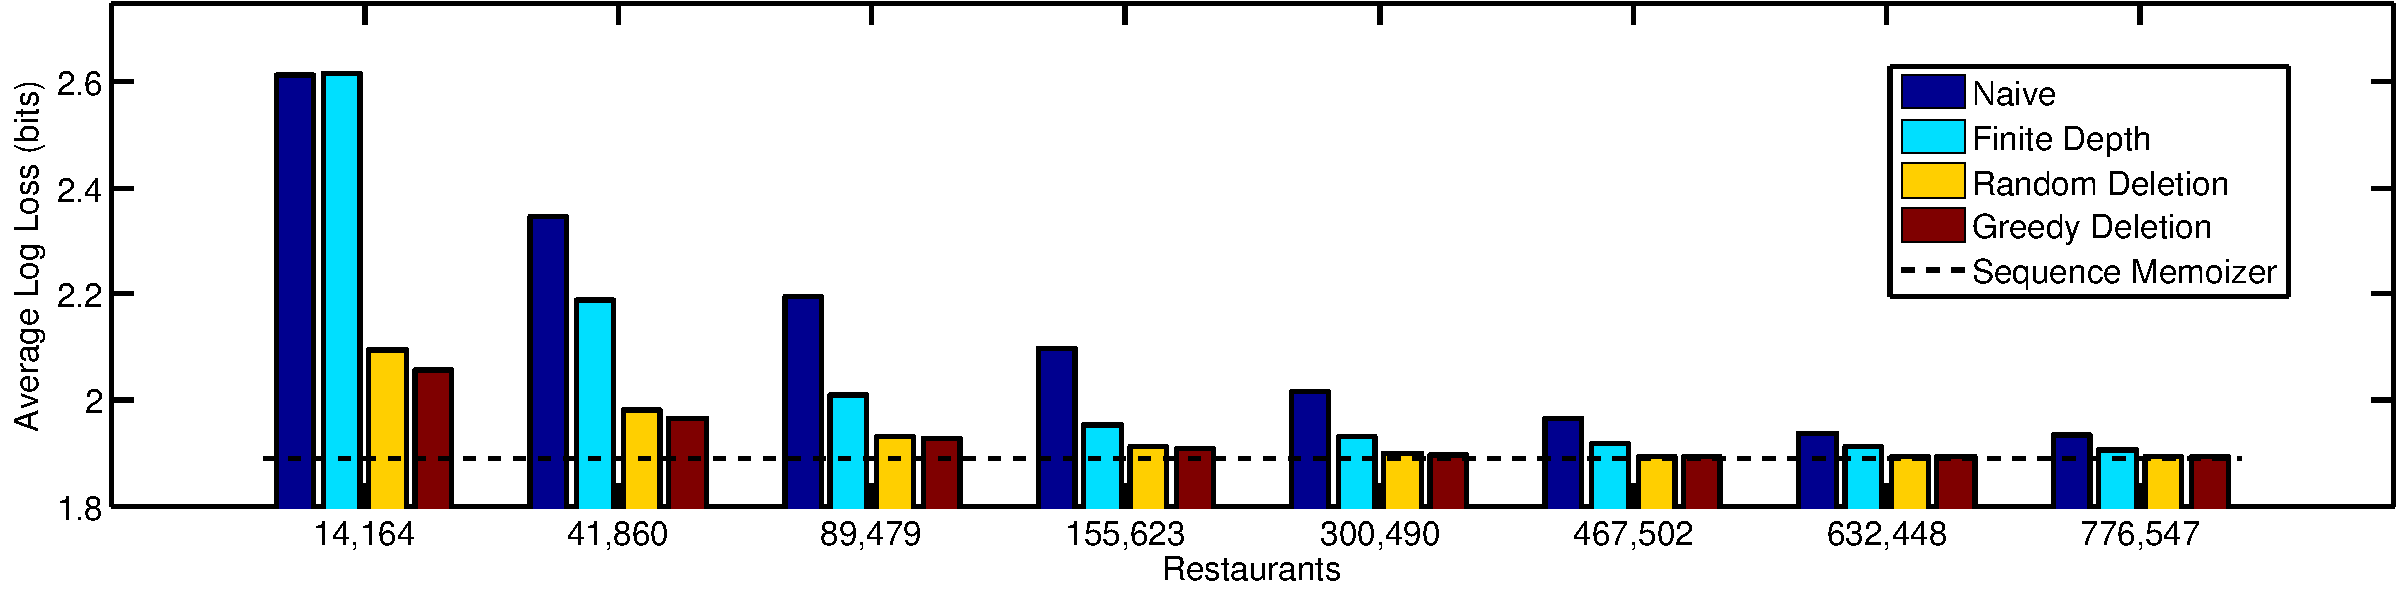
\includegraphics{results_calgary_corpus.pdf}} % [clip=true, viewport= 1in 1in 9in 9in]
		\caption{An example of the possible evolution of the restaurant states in a hierarchical setting}
		\label{figResultsCC}
	\end{center} 
\end{figure*} 

Most steps of the particle filter are based on a sequential estimation approach for the SM proposed in \cite{Gasthaus2010}.  However, this inferential procedure must include the deletion step characteristic of the generative model.  When state of the model represented in each particle reaches the memory constraint we will need to propose values for the the latent parameters indicating which restaurants were deleted. We suggest two different proposal distributions to correspond with the two interpretations of the model specification already discussed.  The first is complementary to the understanding of the model as a sequence of dependent distributions with Pitman-Yor process distributions which vary sequentially across the sequence.  The second is complementary to the understanding of the model as a finite state approximation of a model representation which grows linearly as a function of the length of the data.

The first proposal distribution for the deletion of restaurants is uniform over the leaf nodes of the current state of the model.  Using the generative process as the proposal distribution is standard in particle filtering approaches \cite{Doucet2001}.  We refer to the use of this proposal distribution as using a random deletion scheme.

For the second proposal distribution we note that a fixed state of the model represents a likelihood. We can use this likelihood to approximate the probability of observing the sequence we used to to build the model.  Furthermore, by deleting different leaf restaurants the probability of the sequence, given the updated state of the model, changes, and can be approximated in the same way.  The second proposal distribution deterministically proposes the leaf restaurant whose deletion least negatively impacts the estimated likelihood of the observed sequence.  We refer to the use of this proposal distribution as using a greedy deletion scheme. 

%While the sequential nature of particle filtering fills the incremental requirement, a particle filter with a large particle swarm could still require too much space.  It is possible to implement particle filtering algorithms where the aspects of the particles which overlap are represented only once and thus induce memory savings.  Using such an algorithm here could be extremely complicated.  We suggest the alternative approach of only using one particle in the particle filter.  This approach was shown to be effective in practice by \cite{Gasthaus2010} and simplifies implementation a great deal.


%\subsection{Complexity}

%A little consideration will show that both of the algorithms suggested for inference in this model require constant space, in the sense of the turing machine, and linear time.  The claim that the algorithms are linear in time stems from the fact that each observation must be seated, but now each seating operation is a constant time operation as the length of any path one must traverse in order to seat an observation is bounded by the total number of instantiated restaurants.  Furthermore, each deletion step requires, at worst, visiting every instantiated restaurant, which if done recursively is a constant time algorithm given that the number of instantiated restaurants is limited.  

%The claim that the algorithm requires constant space requires a little more thought.  It is clear that we have limited the space required by restaurant objects, but what about the actual construction of the tree?  Currently our implementation labels each edge between nodes with two integers which index into the original sequence in order to describe that particular edge.  That is, if the parent restaurant corresponds to the distribution over bytes following $oc$,  and the child restaurant corresponds to the distribution over bytes following $acdoc$, the connecting path may be described by the integer array $[17,20]$ if in the sequence being seated, the entries 18-20 are $acd$.  This type of algorithm requires only constant space for each edge, though it works best if the entire sequence is held in memory.  That being said, considering the sequence being seated to be a semi-infinite tape as in the turing machine stipulation, reversals of the tape are allowable.  Thus, the entire sequence need not be held in memory, it is only necessary that we can reverse the tape to access previous entries in the sequence if we need them.

%As a practical side note, an alternative approach to implementation could store the full connecting context on the edge between nodes.  In the above example this would correspond to labeling the edge with the byte array $[acd]$.  While this does not theoretically require constant space, typically when implementing the algorithm on real data only a short section at the end the array is used.  Caching a fixed length section of the each array on the appropriate edge could drastically reduce the number of times the algorithm requires the tape to reverse.  As an example, if one was fitting the entire model on each document of the calgary corpus separately, as we do in the results section, and were willing to cache arrays of length 6,000, a tape reversal would never be required.  This number could only decrease using either of the deletion schemes suggested.  Finally, if we use a fixed depth model, caching the contexts on the edges requires only constant memory when enforcing an upper bound on the number of restaurants.
